\documentclass[12pt]{article}
\usepackage{geometry}
\usepackage{amsmath}
\usepackage{graphicx}
\usepackage{mathptmx}
\usepackage{setspace}
\onehalfspacing
\geometry{a4paper, margin=1in}
\setlength{\parindent}{0pt}
\setlength{\parskip}{1em}

\title{
\includegraphics{9.4.png}\\ IE407 - Homework 1 Report}
\author{Burak Yıldız - 2449049 \\ Ülkü Aktürk - 2450062}
\date{Due Date: 23.03.2024}

\begin{document}

\maketitle
\newpage
\section*{Question 1: Optimal Shoe Production Strategy}

\subsection*{Linear Programming Model}

The linear programming model for minimizing the cost is defined as follows:

Objective Function:
\begin{equation*}
    \text{Minimize } C = 3x_1 + x_2
\end{equation*}

Subject to:
\begin{align*}
    x_1 &\geq 500 &\text{(Hiking shoe demand constraint)} \\
    x_1 + x_2 &\leq 5000 &\text{(Total production capacity constraint)} \\
    \frac{2x_1}{100} + \frac{x_2}{100} &\leq 40 &\text{(Labor force constraint)} \\
    0.2x_1 + 0.5x_2 &\leq 500 &\text{(Cotton material constraint)} \\
    x_1, x_2 &\geq 0 &\text{(Non-negativity constraint)}
\end{align*}

\subsection*{Solution and Analysis}

Using graphical analysis and optimization techniques, we determined the optimal solution for the production of hiking and sprint shoes. The optimal solution is to produce exactly 500 pairs of hiking shoes (\(x_1^*\)) and no sprint shoes (\(x_2^*\)), with a minimum total production cost of \$1500.

\subsection*{Graphical Representation of the Solution}

\begin{figure}[h!]
    \centering
    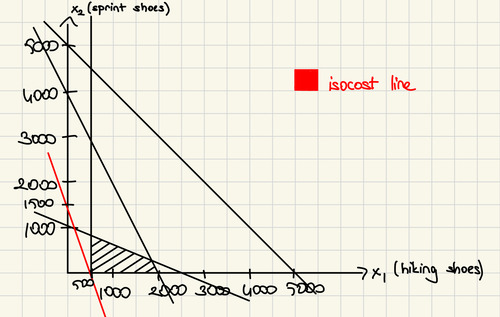
\includegraphics[width=0.8\textwidth]{urban-3-dijital-2-1 2-2.jpeg}
    \caption{Feasible Region for Shoe Production}
\end{figure}

\subsection*{Constraints}
\begin{align*}
    x_1 &\geq 500 &\text{Binding constraint} \\
    x_1 + x_2 &\leq 5000 &\text{Redundant constraint} \\
    \frac{2x_1}{100} + \frac{x_2}{100} &\leq 40 &\text{Non-binding constraint} \\
    0.2x_1 + 0.5x_2 &\leq 500 &\text{Non-binding constraint} \\
    x_1&\geq 0 &\text{Non-binding constraint} \\
    x_2 &\geq 0 &\text{Binding constraint} 
\end{align*}

\subsection*{Scenarios Analysis}

\subsubsection*{Increase in the Cost of Sprint Shoes}

The increase in the cost of producing sprint shoes does not affect the current optimal solution since it involves producing only hiking shoes. The cost of sprint shoes can increase until other constraints become limiting factors before the cost makes producing sprint shoes unfeasible.

\subsubsection*{Increase in Demand for Hiking Shoes}

The maximum increase in demand for hiking shoes that can be supported without changing the current optimal solution is an additional 1500 pairs. This indicates that the demand for hiking shoes can increase to up to 2000 pairs without necessitating a change in the production strategy, given the constraints on labor and cotton availability.

\section*{Conclusion}

The analysis provides a clear strategy for Tasch Co. to minimize production costs while meeting demand and resource constraints. By focusing on the production of hiking shoes and considering the flexibility in adjusting to increased demand or changes in production costs, Tasch Co. can efficiently manage its shoe production operations.


\section*{Question 2: Optimal Strategy for Oil Products}

\subsection*{Introduction}
This report presents an analysis aimed at determining the optimal production levels of high emission (LE) and clean emission (CE) oil products to maximize the weekly revenue for Küpraş refinery. The problem is constrained by the production capacities and demands for both products.

\subsection*{Linear Programming Model}
The linear programming model was formulated with the objective to maximize the revenue from selling LE and CE oil products, considering constraints on production capacity, material availability, and product demands.

\subsection*{Solver Setup}
Excel Solver was configured to maximize the objective function $Z = 40 \times \text{Total\_LE} + 70 \times \text{Total\_CE}$, subject to the constraints provided in the sensitivity report.

\subsection*{Results}
According to the Solver's optimal solution, the refinery should produce 60,000 barrels of LE and 90,000 barrels of CE to achieve maximum revenue under the given constraints. The amount of CO needed for LE is 30714.2857 , the amount of HO needed for LE is 29285.7143. The amount of CO needed for CE is 19285.7143 , the amount of HO needed for CE is 70714.2857. 

\subsection*{Sensitivity Analysis}
The sensitivity report reveals that the price of LE can increase by up to \$30 without changing the optimal basis of the solution. Conversely, the price can decrease by \$40 before the solution changes, indicating a range of \$[0, 70]\$ for the price of LE within the current optimal basis.

\subsection*{Price Increase Impact}
With an allowable increase of \$30 in the price of LE, increasing the price by \$1 (from \$40 to \$41) will not change the optimal production quantities. However, it will increase the total revenue by \$60,000, given that the shadow price for LE production is \$0. This implies that within the current optimal solution space, there's a buffer to increase the price of LE without affecting the production strategy.



\subsection*{Price of CE Analysis}

The allowable increase for the price of Clean Emission (CE) oil is extremely high, indicating that the price can be increased indefinitely without affecting the optimal basis. The allowable decrease is \$30, suggesting that the price of CE can be reduced to \$40 per barrel before the optimal solution changes. Therefore, the current optimal production levels of 60,000 barrels for LE and 90,000 barrels for CE will remain unchanged for any price increase of CE.

Increasing the price of CE by \$1 per barrel, within the infinite allowable increase range, will not alter the production quantities. It will, however, result in an increased revenue of \$90,000, reflecting the additional \$1 per barrel over 90,000 barrels. Conversely, decreasing the price by \$10 per barrel will reduce the total revenue by \$900,000 but will not affect the production strategy.


% ... (previous content)

\subsection*{Warehouse Space of CO Analysis}

The sensitivity report indicates that the shadow price for warehouse space of CO is \$40 per barrel, with an allowable increase in warehouse space of 27,857 barrels and an allowable decrease of 15,000 barrels. This suggests that the warehouse capacity can be reduced by 15,000 barrels without affecting the current optimal production levels. However, any increase beyond 27,857 barrels would necessitate a reevaluation of the production strategy.

Considering the shadow price, the most Küpraş should be willing to pay to expand the warehouse space by 1,000 barrels is \$40,000, With an increase of 80,000 barrels, since this increase is more than allowable increase re-optimization is required.

After increasing the warehouse capacity for CO by 80,000 barrels, the production of LE has increased remarkably to 110,000 barrels, exploiting the additional CO capacity. The optimization also adjusted the CE production, slightly reducing it to 80,606.06 barrels.

This expansion of warehouse space has resulted in a considerable increase in the objective function value, from \$8,700,000 to over \$10,042,424.24. The model now utilizes 90,606.06 barrels of the available 130,000 barrels of CO.


% ... (remainder of the document)

% ... (previous content)

\subsection*{Analysis of Minimum Delivery Requirement of LE}

The sensitivity report indicates that the minimum delivery requirement for LE can be adjusted without affecting the current optimal solution, as long as the adjustment falls within the range allowed by the sensitivity analysis. The shadow price for the LE production constraint is \$0, signaling that the objective function value does not improve or worsen with marginal changes to the LE production level within the allowable range.

Given that the shadow price is \$0, when the minimum delivery requirement of LE is increased by 3,000 barrels per week, knowing this is within the allowable increase 15000, there will be no impact on the revenue. The production plan would remain at 110,000 barrels of LE, with the same associated revenue, suggesting that there is flexibility in the production capacity to accommodate an increase in LE demand.

The findings indicate that Küpraş has the operational flexibility to increase the minimum delivery requirement for LE by 3,000 barrels without incurring additional costs or losing revenue, thus maintaining the current basis for optimal production.

% ... (remainder of the document)



\end{document}
